\chapter{Project Management}
\label{project management}

\section{The Group}
The group formed out of the desire to work together based on varying levels of previous experience working together, rather than out of a desire to work on a specific project as was the case with other groups.
The group quickly decided to take advantage of the new iLab at Warwick University \cite{Kalvala2013} and chose to make use of the Microsoft Kinect.
Initial ideas revolved around object modelling and sharing, but due to the low resolution and minimum scanning distance of the Kinect, these early ideas were abandoned.
After discussions with the project supervisor, the group chose to tackle the problem proposed by \todo{the italians}.\\

\begin{figure}[h]
\begin{center}
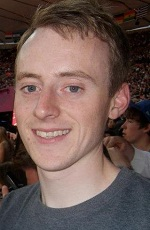
\includegraphics[scale=0.5]{./pm/bernard}
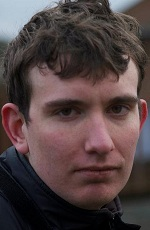
\includegraphics[scale=0.5]{./pm/greg}

\includegraphics[scale=0.5]{./pm/nathan}

\includegraphics[scale=0.5]{./pm/robin}

\includegraphics[scale=0.5]{./pm/stef} 
\end{center}
\caption{The group from left to right: Bernard, Greg, Nathan, Robin and Paps.}
\label{fig:the group}
\end{figure}

\section{Group Behaviour}

\subsection{Weekly Meetings}
The group quickly took to organising weekly meeting. 
In these meetings, progress of previous weeks activities could be ascertained and if necessary, more resources added to a outstanding task to ensure it's timely completion. 
If the previous weeks tasks had been completed, a new task for the upcoming week would be assigned to group members during this time.\\

\subsection{Group Coding Sessions}
Often, the group would congregate around the Kinect in CS0.01 within the Computer Science Department at Warwick to work on the project. The group would use these occasions to provide fresh insight into individual problems and was often the setting for the peer review process.\\

\subsection{Peer Review Process}
\label{pm:peer review process}
Regularly, the group would informally demo the latest work to the group.
These demos gave the opportunity for the group to feedback and comment on any assumptions that had been made to get the section working, such as the volume estimator assuming the person is an amorphous blob.\\

\subsection{Centralised Code Repository}
The group made use of a Git repository to manage source code, which whilst it had a steep learning curve, has avoided any version control issues.\\

\subsection{Self organising Sub Committees}
Often, once tasks had been allocated, the group would subdivide into sub committees and work on tasks together. 
This division meant that a subset of the group could focus on one particular problem in isolation.\\

\subsection{Clear Task Responsibility}
As a result of the weekly meetings, each group member was assigned a task weekly and as such each member had a clear responsibility for there given task.\\

\subsection{Morale}
\label{morale}
In order to maintain a high group morale, many "memes" were created out of the group to lift spirits and keep humour present after particularly tense group meetings. A selection is reproduced in Figures \ref{fig:were_meeting_now?} through to \ref{fig:sexy_sexton}

\begin{figure}[h]
\begin{center}
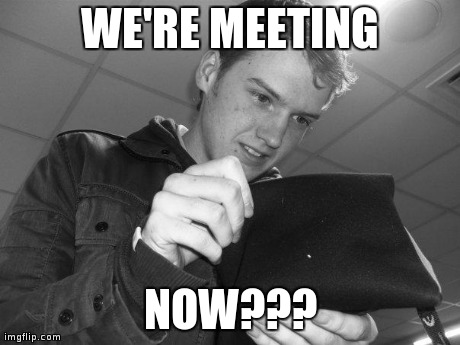
\includegraphics[scale=0.4]{./design/nathan} 
\end{center}
\caption{We're meeting now?}
\label{fig:were_meeting_now?}
\end{figure} 

\begin{figure}[h]
\begin{center}
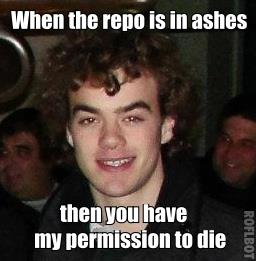
\includegraphics[scale=0.4]{./design/banerobin}
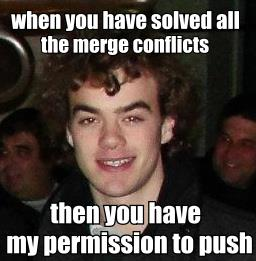
\includegraphics[scale=0.4]{./design/banerobin2}  
\end{center}
\caption{Good guy / Scum bag Robin}
\label{fig:scum_bag_robin}
\end{figure}

\begin{figure}[h]
\begin{center}
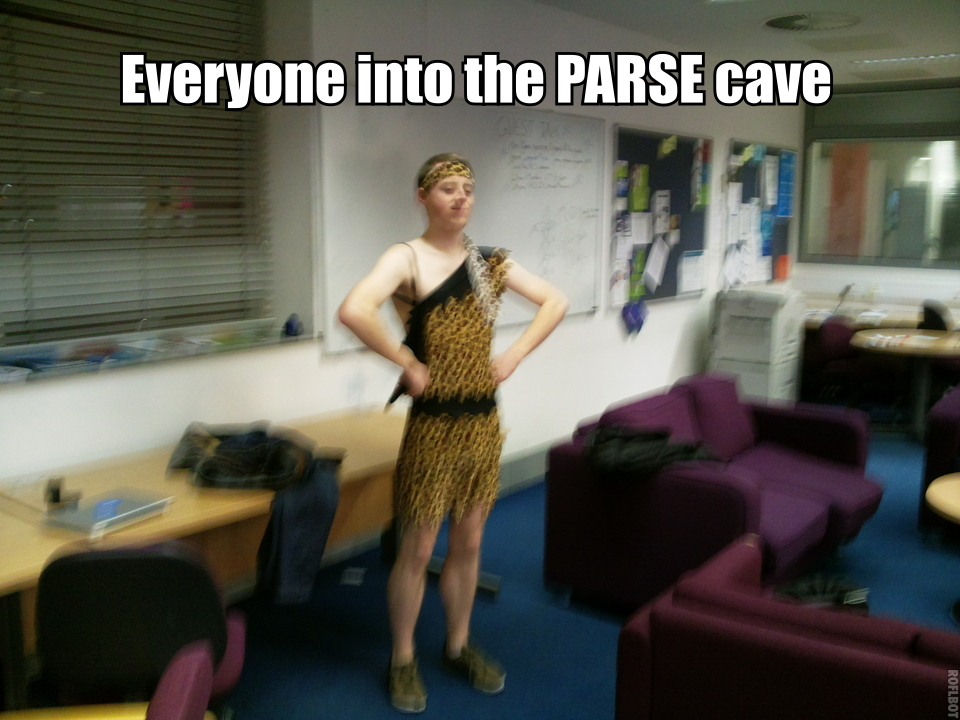
\includegraphics[scale=0.4]{./design/PARSECave} 
\end{center}
\caption{Sexy Sexton}
\label{fig:sexy_sexton}
\end{figure} 